\documentclass[10pt]{extarticle}
\title{}
\author{}
\date{}
\usepackage[shortlabels]{enumitem}


%paper setup
\usepackage{geometry}
\geometry{letterpaper, portrait, margin=1in}
\usepackage{fancyhdr}
% sans serif font:
\usepackage{cmbright}
%symbols
\usepackage{amsmath}
\usepackage{amssymb}
\usepackage{amsthm}
\usepackage{mathtools}
\usepackage[hidelinks]{hyperref}
\usepackage{gensymb}
\usepackage{multirow,array}
\usepackage{multicol}

\newtheorem*{remark}{Remark}
\usepackage[T1]{fontenc}
\usepackage[utf8]{inputenc}

%chemistry stuff
%\usepackage[version=4]{mhchem}
%\usepackage{chemfig}

%plotting
\usepackage{pgfplots}
\usepackage{tikz}
\tikzset{middleweight/.style={pos = 0.5}}
%\tikzset{weight/.style={pos = 0.5, fill = white}}
%\tikzset{lateweight/.style={pos = 0.75, fill = white}}
%\tikzset{earlyweight/.style={pos = 0.25, fill=white}}

%\usepackage{natbib}

%graphics stuff
\usepackage{graphicx}
\graphicspath{ {./images/} }
\usepackage[style=numeric, backend=biber]{biblatex} % Use the numeric style for Vancouver
\addbibresource{the_bibliography.bib}
%code stuff
%when using minted, make sure to add the -shell-escape flag
%you can use lstlisting if you don't want to use minted
%\usepackage{minted}
%\usemintedstyle{pastie}
%\newminted[javacode]{java}{frame=lines,framesep=2mm,linenos=true,fontsize=\footnotesize,tabsize=3,autogobble,}
%\newminted[cppcode]{cpp}{frame=lines,framesep=2mm,linenos=true,fontsize=\footnotesize,tabsize=3,autogobble,}

%\usepackage{listings}
%\usepackage{color}
%\definecolor{dkgreen}{rgb}{0,0.6,0}
%\definecolor{gray}{rgb}{0.5,0.5,0.5}
%\definecolor{mauve}{rgb}{0.58,0,0.82}
%
%\lstset{frame=tb,
%	language=Java,
%	aboveskip=3mm,
%	belowskip=3mm,
%	showstringspaces=false,
%	columns=flexible,
%	basicstyle={\small\ttfamily},
%	numbers=none,
%	numberstyle=\tiny\color{gray},
%	keywordstyle=\color{blue},
%	commentstyle=\color{dkgreen},
%	stringstyle=\color{mauve},
%	breaklines=true,
%	breakatwhitespace=true,
%	tabsize=3
%}
% text + color boxes
\renewcommand{\mathbf}[1]{\mathbold{#1}}
\usepackage[most]{tcolorbox}
\tcbuselibrary{breakable}
\tcbuselibrary{skins}
\newtcolorbox{problem}[1]{colback=white,enhanced,title={\small #1},
          attach boxed title to top center=
{yshift=-\tcboxedtitleheight/2},
boxed title style={size=small,colback=black!60!white}, sharp corners, breakable}
%including PDFs
%\usepackage{pdfpages}
\setlength{\parindent}{0pt}
\usepackage{cancel}
\pagestyle{fancy}
\fancyhf{}
\rhead{Avinash Iyer}
\lhead{Math 400: Homework 8}
\newcommand{\card}{\text{card}}
\newcommand{\ran}{\text{ran}}
\newcommand{\N}{\mathbb{N}}
\newcommand{\Q}{\mathbb{Q}}
\newcommand{\Z}{\mathbb{Z}}
\newcommand{\R}{\mathbb{R}}
\begin{document}
  \begin{problem}{4}
    Show that Corollary 10.3 cannot be improved by giving an example of a planar graph that contains no vertex of degree $4$ or less.
    \tcblower
    \begin{center}
      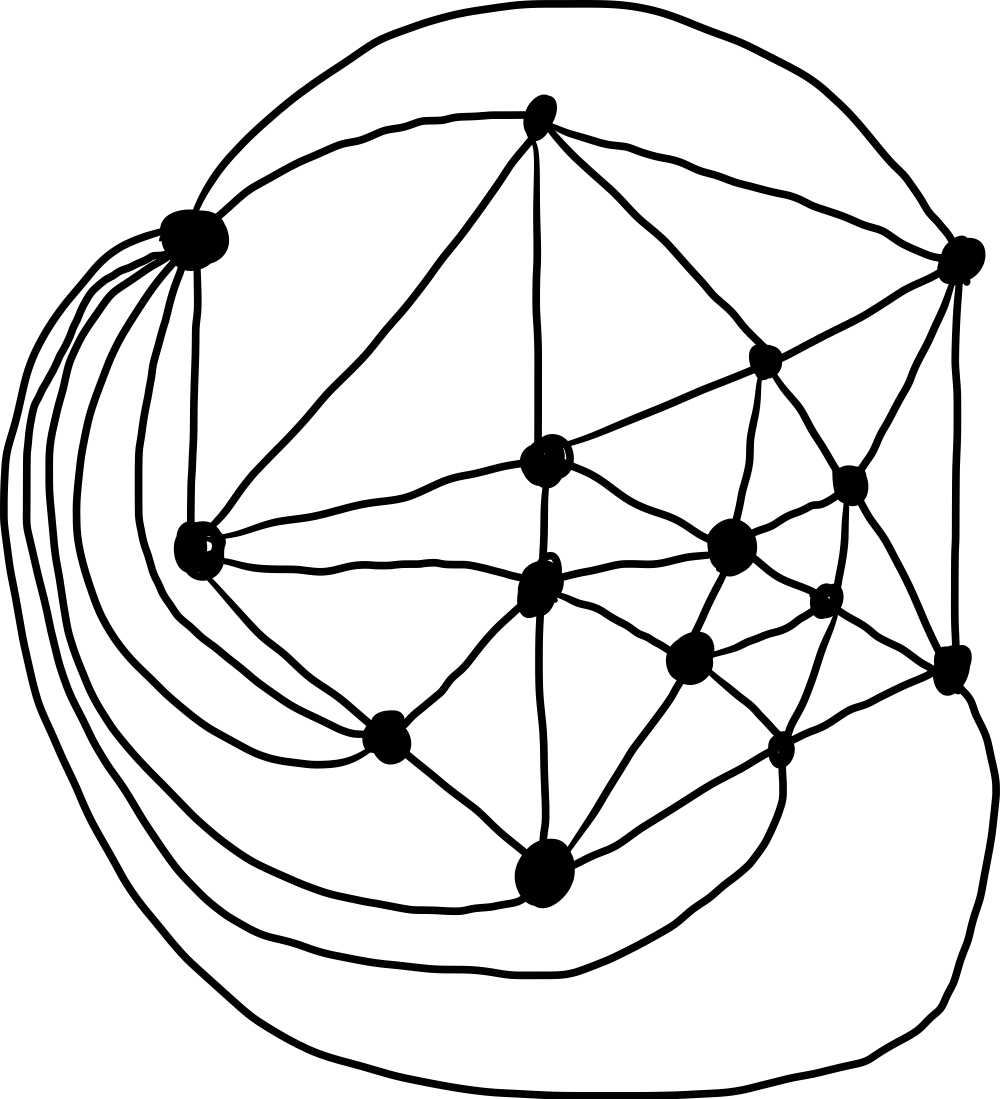
\includegraphics[width=0.4\textwidth]{images/10_4_sol.png}
    \end{center}
  \end{problem}
  \begin{problem}{5}
    \begin{enumerate}[(a)]
      \item Show that the Petersen graph does not contain a subdivision of $K_5$.
      \item Show that the Petersen graph is nonplanar.
    \end{enumerate}
    \tcblower
    \begin{problem}{(a)}
      Since all the vertices of the Petersen graph are of degree $3$, and any subdivision of $K_5$ must contain a vertex of at least degree $4$, this means the Petersen graph cannot contain a subdivision of $K_5$.
    \end{problem}
    \begin{problem}{(b)}
      Suppose that the Petersen graph is planar. Then, by Euler's formula,
      \begin{align*}
        (10) - (15) + F = 2,
      \end{align*}
      meaning there are $7$ faces. However, since the girth of the Petersen graph is $5$, this means every face in the supposed planar configuration is made of pentagons --- implying that the Petersen graph must have at least $\lfloor35/2\rfloor$ or $17$ edges. $\bot$
    \end{problem}
  \end{problem}
  \begin{problem}{6}
    Does there exist a $4$-regular planar graph of order $7$?
    \tcblower
    \begin{center}
      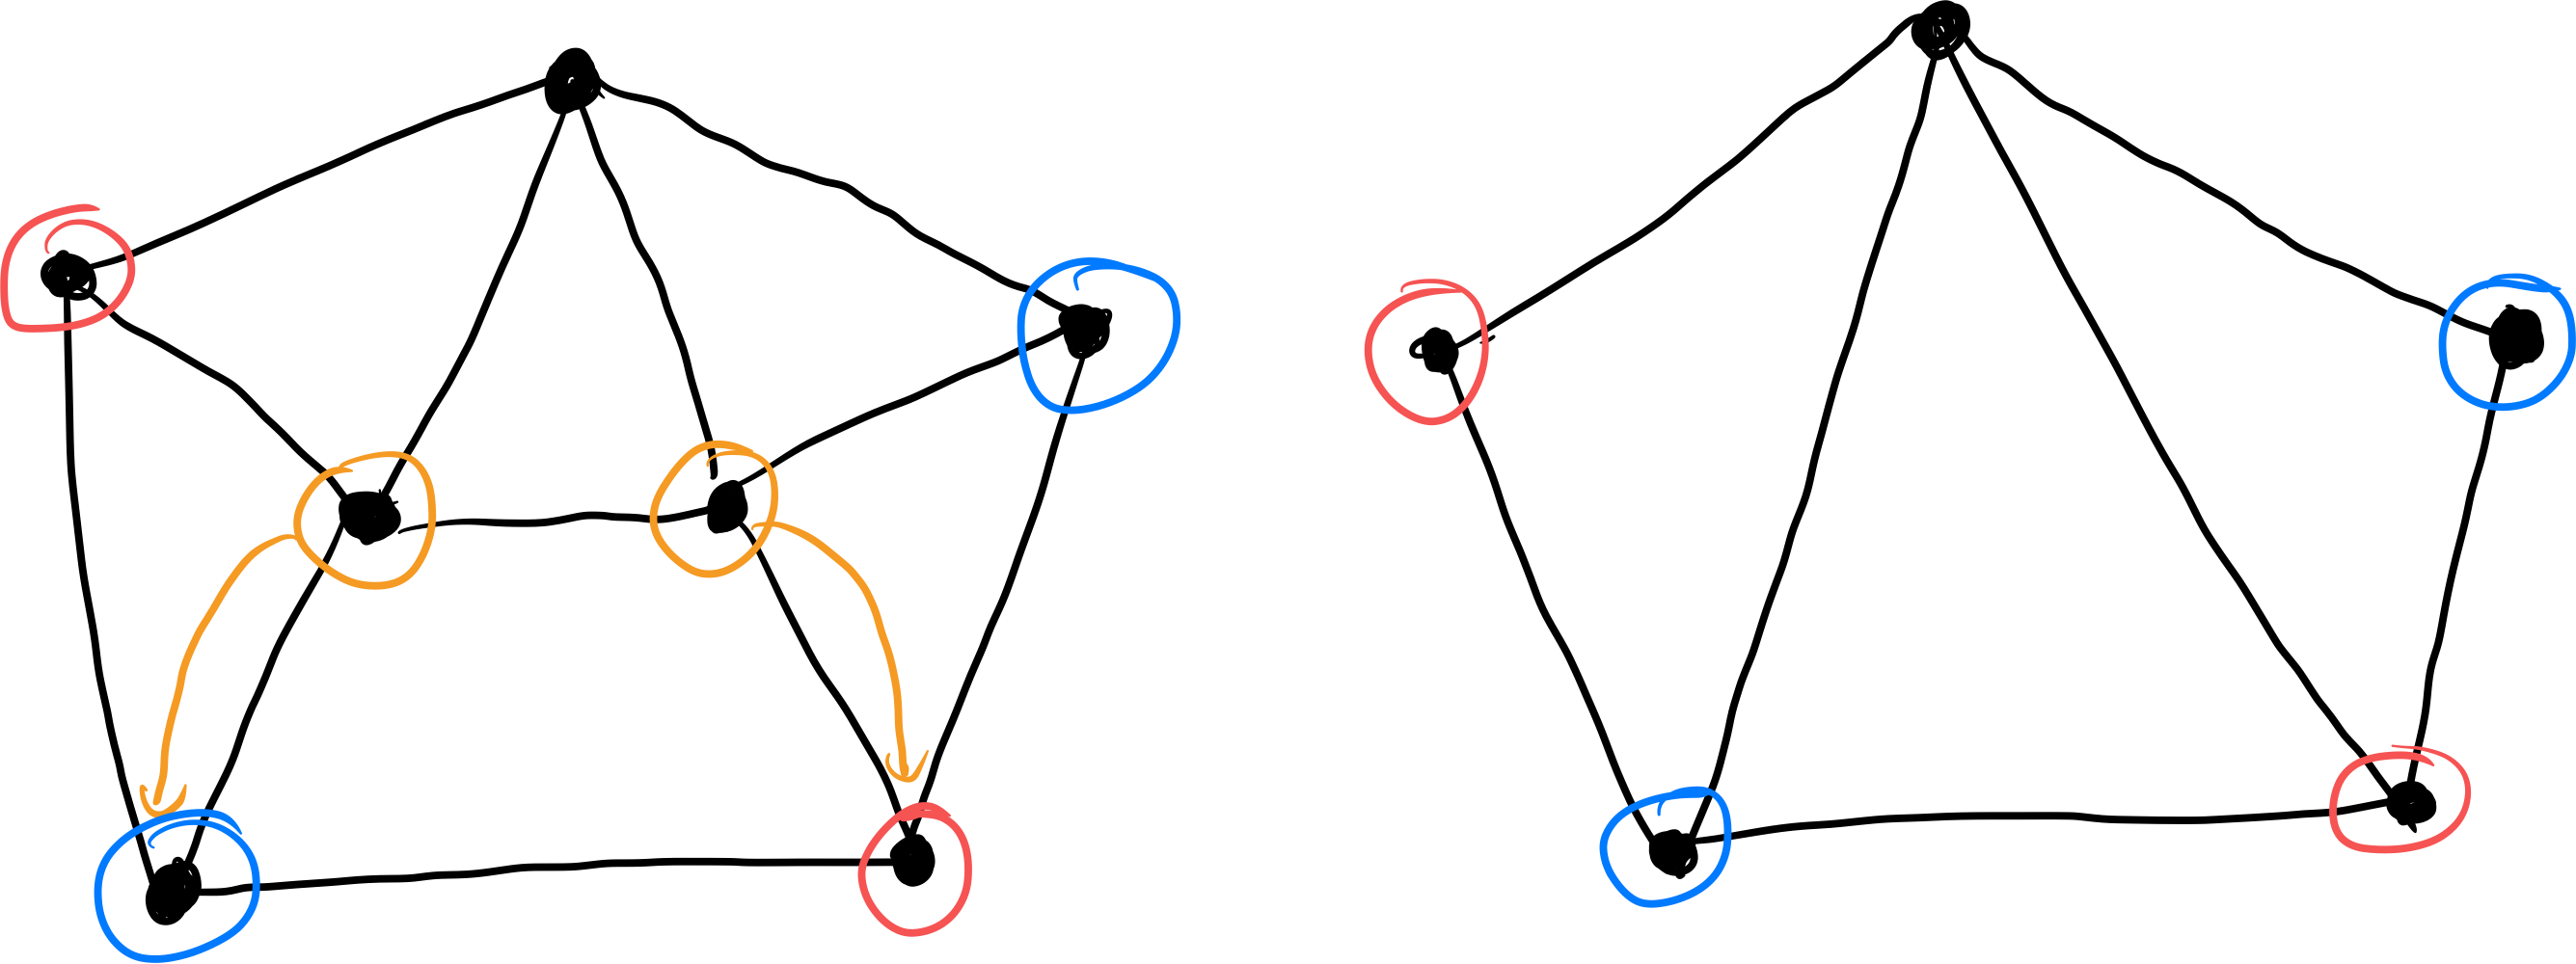
\includegraphics[width=0.5\textwidth]{images/10_6_sol.png}
    \end{center}
    In the left image above of an incomplete construction of our supposed planar $4$-regular graph of order $7$, we see that the blue vertices still require an edge between them, and similarly, the red edges still require an edge between them.\\

    Creating a minor by retracting the two orange vertices using the above arrows, we see that the connection would yield a graph of $K_5$ --- and since $K_5$ is a minor of our $4$-regular graph of order $7$, by Wagner's theorem, it must be non-planar.
  \end{problem}
  \begin{problem}{7}
    Find all graphs $G$ of order $n\geq 5$ and size $m = 3n-5$ such that $G-e$ is planar for every edge $e$ of $G$.
    \tcblower
    I don't know how to do this problem.
  \end{problem}
  \begin{problem}{8}
    Find all cycles $C_n$ of order $n\geq 3$ for which $\overline{C_n}$ is a nonplanar graph.
    \tcblower
    The following graphs are planar:
    \begin{itemize}
      \item $\overline{C_3}$ is three vertices without any edges.
      \item $\overline{C_4}$ is two disconnected $K_2$ graphs.
      \item $\overline{C_5}$ is one-to-one with $C_5$
      \item $\overline{C_6}$ is planar:
        \begin{center}
          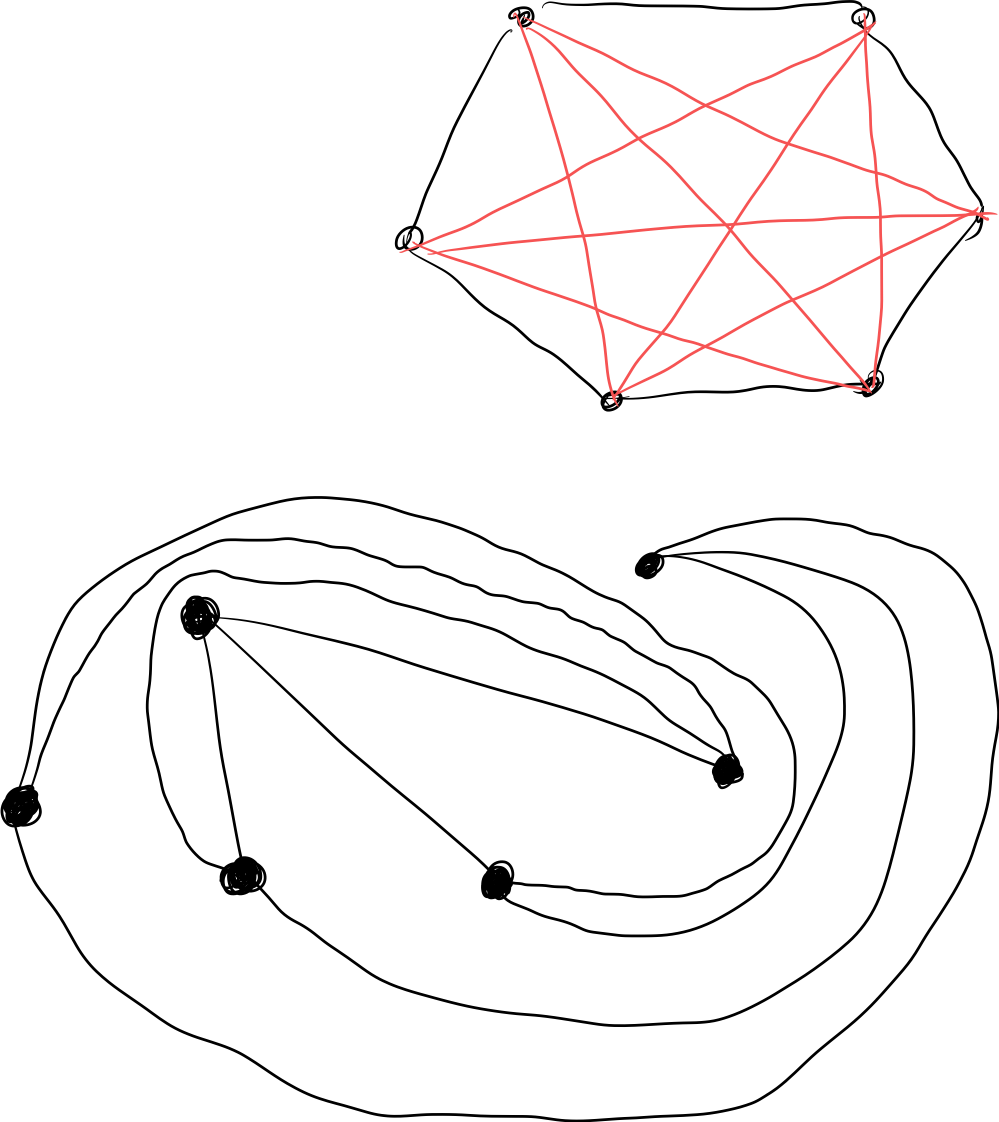
\includegraphics[width=0.5\textwidth]{images/10_8_sol.png}
        \end{center}
    \end{itemize}
    For $n = 7$, $ \overline{C_7} $ must be a $4$ regular graph of order $7$, which we showed was nonplanar.\\

    For every $n\geq 8$, $|E(\overline{C_n})| = \frac{n(n-3)}{2} > 3n-6$.\\

    Therefore, $\overline{C_n}$ is nonplanar for every $n\geq 7$.
  \end{problem}
  \begin{problem}{18}
    Show that both $K_{5}$ and $K_{3,3}$ are minors of the graph $G$ in Figure 10.13
    \tcblower
    I don't know how to do this problem.
  \end{problem}
  \begin{problem}{19}
    Suppose that a connected graph $H$ is a minor of a tree $T$. Show that $H$ is also a tree.
    \tcblower
    Let $T$ be a tree. Then, $|E(T)| = n-1$, where $n = |V(T)|$. For any contraction performed on $T$ in the process of yielding $H$, it must be the case that both $|E(T)|$ and $|V(T)|$ are reduced by the same quantity --- thus, $|E(H)| = k-1$ where $k = |V(H)|$.
  \end{problem}
\end{document}
